\documentclass[10pt,showpacs,preprintnumbers,footinbib,amsmath,amssymb,aps,prl,twocolumn,groupedaddress,superscriptaddress,showkeys]{revtex4-1}
\usepackage{graphicx}
\usepackage{dcolumn}
\usepackage{bm}
\usepackage[colorlinks=true,urlcolor=blue,citecolor=blue]{hyperref}
\usepackage{color}
\usepackage{listings}
\usepackage{amsmath}
\usepackage{subcaption}
\usepackage{hyperref}
\usepackage{fancyref}
\usepackage{verbatim}

\begin{document}



\title[CPP2]{Computational Physics Project 3\\
\large{The Solar System}\\
or\\
I can See my House from Here!}

\author{Marius B. Pran}
\affiliation{Institute of Theoretical Astrophysics, University of Oslo}
\author{Espen Hodne} 
\affiliation{Institute of Theoretical Astrophysics, University of Oslo}
\author{Marc K. Pestana}
\affiliation{Institute of Theoretical Astrophysics, University of Oslo}


\begin{abstract}


\end{abstract}



\maketitle



\section{Introduction}

The solar system is our local stellar system, and has been of an interest to humanity for ages. During our history a great number of models has been proposed, until we finally landed on one with the Sun in the middle and the planets orbiting it. In this project we make a model of this system, using Newton's law of gravitational force between each celestial object. We make the initial assumption that the Sun is the centre-of-mass, and that we have circular orbits. We then let every celestial object in the system affect one another gravitationally and see what happens, with the goal of getting a stable and semi-realistic solar system model.

In this project we use numerical methods to make a model of the solar system. Specifically we use the velocity Verlet method to calculate the planetary orbits, as it does not entail the kind of evolving uncertainties one finds in the standard forward Euler.



\section{Methods and Algorithms}

\subsection{Overview}

The methods used is an object-oriented program, with separate classes for celestial objects, calculating energy and momentum etc. The program was in large part written by Anders Hafreager, and modified further by us.

The most important formula we use is Newton's law of gravitation

\begin{equation}
F_G = \frac{G M_1 M_2}{r^2}
\end{equation}

where $G$ is the universal gravitational constant, $M_1$ and $M_2$ are the masses of two objects and $r$ is the distance between the objects. Our main principle is that we let this force work between a number of celestial objects, give each object a starting position and velocity and let the program run for a pre-decided time period.

For most of the project we assume the Sun is standing still in the system origin at the outset. Thus, the only movement of the Sun comes from the gravitational pull of the planets. However, towards the end, when we plot the entire solar system, we will give the Sun a new initial position and velocity gathered from NASA's websites. We will get the initial data for the planets the same way.


\subsection{The Forward Euler and Velocity Verlet Methods}


In this project we are using two different numerical integration methods: the forward Euler method and the velocity Verlet method.


At first, we want to test the methods using circular velocities for our planets. This is fairly simple to achieve, we just place the planet purely in the x-direction and then give it an y-velocity of $v_y = 2\pi r/t_{orb}$. Here $r$ is the distance between the Sun and the planet, and $t_{orb}$ is the orbital period.

The forward Euler method is perhaps the most well-known and basic method of numerical integration. It is intuitive, simple, effective and disturbingly unprecise.

The forward Euler method (in our case) is given as 

\begin{equation}
v_{i+1} = v_i + a_i dt
\end{equation}

\begin{equation}
r_{i+1} = r_i + v_i dt
\end{equation}

where $r_i$ is the position in our current step, $v_i$ the velocity, $a_i$ the acceleration and $dt$ the size of our time-step. $a$ is gained from Newton's second law, wich states that 

\begin{equation}
\Sigma F = M\textbf{a}
\end{equation}

where $\Sigma F$ is the sum of all forces acting on an object, $M$ is the object's mass and $a$ its acceleration.

Since both the force acting on each celestial object and their masses are known quantities, we then get the acceleration by 

\begin{equation}
a_i = \frac{F_G}{M}
\end{equation}

The velocity Verlet method works a bit differently. We still use that $a_i = \frac{F}{M}$, but for velocity and position we use that 

\begin{equation}
v_{i+1} = v_i + \frac{(a_{i+1} + a_i)}{2}dt
\end{equation}

and 

\begin{equation}
r_{i+1} = r_i +  v_i dt + \frac{a_i}{2}dt^2
\end{equation}

The main difference is that the velocity Verlet method is a second-order method, while the forward Euler is a first-order method. That means the error in the velocity Verlet will be much smaller. In physical problems, this often translates into forward Euler not conserving energy properly (see table \ref{tab:euler_vs_verlet_earth_sun}.

The effect of this can be seen in figure \ref{fig:euler_vs_verlet_5yr}. In subfigures \ref{fig:e_s_euler_5yr_dt0_00001} and \ref{fig:e_s_verlet_5yr_dt0_00001} we use $dt = 0.00001$ for both methods, while subfigures \ref{fig:s_s_euler_5yr_dt0_001} and \ref{fig:s_s_verlet_5yr_dt0_001} use $dt = 0.001$. 




\subsection{The Earth-Sun System}

First we look at the Earth-Sun system. Here we introduce a scaling of our equations that we use for the entire projects. Specifically, radius is given in units of $1\mathrm{AU} = 149 597 870 700\mathrm{m}$, Astronomical Units, which is the average distance between the Sun and the Earth. We also give all masses in $1\mathrm{M_\odot} = 1.9891\times10^{30}\mathrm{kg}$, which is the mass of the Sun.

If we assume the Earth follows a circular motion (which is wrong, but we will assume it anyway) we get that


\begin{equation}
F_G = \frac{G M_\odot M_{Earth}}{r^2} = \frac{M_{Earth}v^2}{r}
\end{equation}

$$
\implies \frac{G M_\odot}{r} = v^2 \implies GM_\odot = v^2 r
$$

$$
v = \frac{2\pi r}{t} \implies v^2 = \frac{4\pi^2 r^2}{t^2} \implies v^2 r = \frac{4\pi^2 r^3}{t^2}
$$

so

\begin{equation}
GM_\odot = \frac{4\pi^2 r^3}{t^2}
\end{equation}

In our chosen units (with $M_\odot = 1$) this means that the gravitational constant is

\begin{equation}
G = 4\pi^2 \mathrm{AU^3/yr^2}
\end{equation}

The results can be seen in figures \ref{fig:euler_vs_verlet_5yr} and \ref{fig:euler_vs_verlet}. 

We write an object-oriented code to handle this system. It runs on the main principle of "write once, run many times." The code consists of classes for celestial objects, the solar system force and energy calculations, the Verlet and Euler methods, one for making 3D vectors, and a "main" class for inputting values for all desired values. The code was written by Anders Hafreager, and modified by us to include energy calcualtions and a velocity Verlet class.

The code works in a way that allows us to give initial conditions for each celestial object, then send those into the classes to get out the energies and update the positions of each object. We can use the same classes for each and every object, which makes it very convenient to extend the code. All we do is create a new object with a new set of initial positions, velocities and mass.

\subsection{Escape Velocity}

In a spherically symmetric example such as this, we can use the regular formula for escape velocity at a point where $K - U = 0$. i.e. the kinetic energy is equal to the gravitational potential energy. This gives us
\begin{align*}
0 &= \frac{1}{2} Mv^2 - \frac{GMM_\odot}{r}\\
v_e &= \sqrt{\frac{2GM_\odot}{r}}\\
G &= 2\pi^2 \mathrm{AU^3yr^{-2}M_\odot^{-1}}\\
r &= 1\mathrm{AU}\\
v_e &= 2\pi
\end{align*}
It is important to note that this velocity is pointed directly away from the Sun, and the initial velocity of the Earth is pointed perpendicular to the initial position of the sun.



\subsection{The Three-Body System}

In the same way that the Earth and the Sun attract each other, they each share a mutual attraction with all other celestial objects. Thus the prescence of other planets should affect the Earth's (and the Sun's) movement and positions. Since Jupiter has more mass than the rest of the planets combined, we add Jupiter to our model to see how it interacts with the Earth and the Sun.

The program we use is easily extendable. Therefore, adding Jupiter to make a three-body system is a simple task.

Using the velocity Verlet algorithm, we plot the orbits over a period of 25 years (which is a little bit more than twice Jupiter's orbital period), with at timestep of $dt = 0.00001$.



\section{Results}



\subsection{Forward Euler vs. Velocity Verlet and the Earth-Sun System}

Figure \ref{fig:euler_vs_verlet_5yr} shows the differences between forward Euler and velocity Verlet over 5 years, using $dt = 0.00001$ and $dt = 0.001$.

\begin{figure}
	\centering
	\begin{subfigure}[b]{0.3\textwidth}
		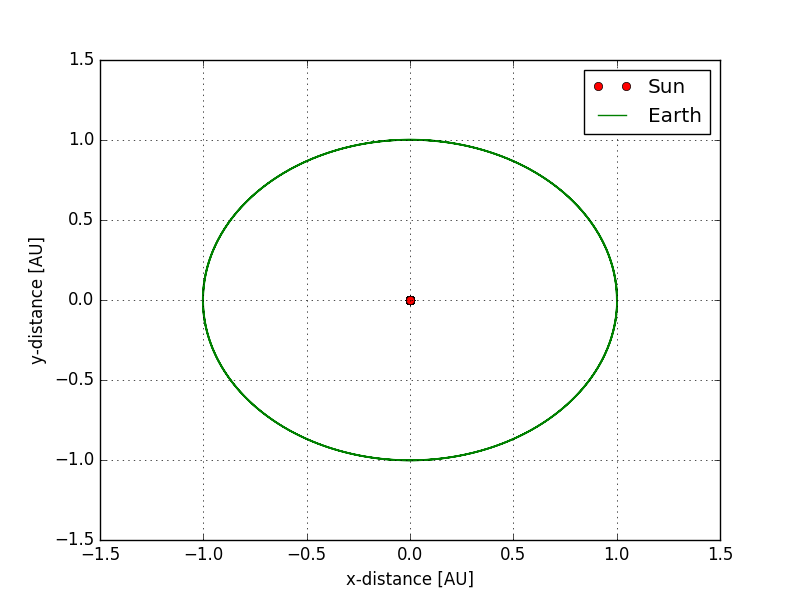
\includegraphics[width=\textwidth]{earth_sun_euler_5years_dt0_00001.png}
		\caption{Earth-Sun system over 5 years, calculated with forward Euler with $dt = 0.00001$.}
		\label{fig:e_s_euler_5yr_dt0_00001}
	\end{subfigure}
    \begin{subfigure}[b]{0.3\textwidth}
		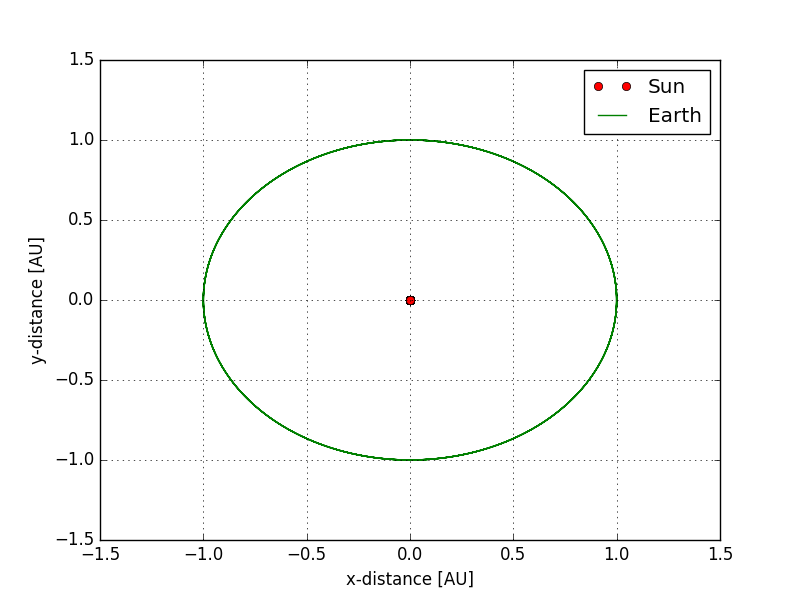
\includegraphics[width=\textwidth]{earth_sun_verlet_5years_dt0_00001.png}
		\caption{Earth-Sun system over 5 years, calculated with velocity Verlet with $dt = 0.00001$.}
		\label{fig:e_s_verlet_5yr_dt0_00001}
	\end{subfigure}
	
	
    \begin{subfigure}[b]{0.3\textwidth}
		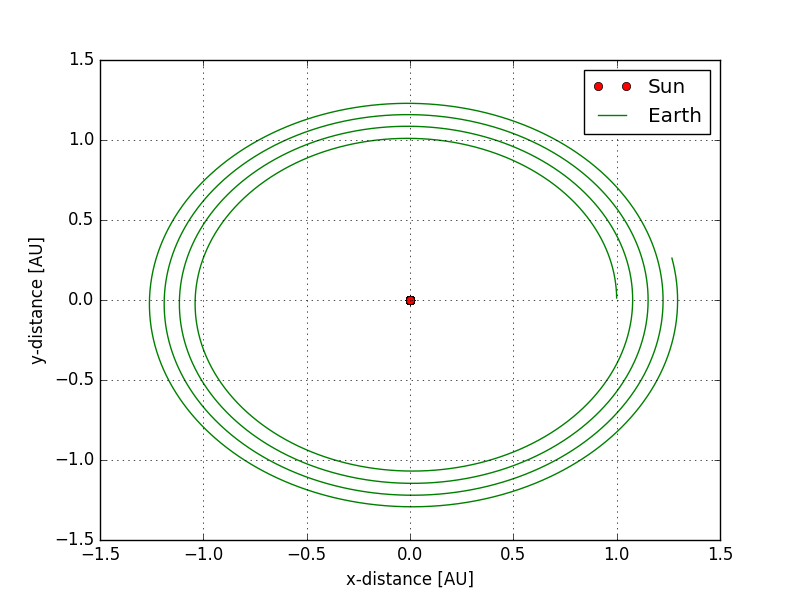
\includegraphics[width=\textwidth]{earth_sun_euler_5years_dt0_001.png}
		\caption{Earth-Sun system over 5 years, calculated with forward Euler with $dt = 0.001$.}
		\label{fig:s_s_euler_5yr_dt0_001}
	\end{subfigure}
	\begin{subfigure}[b]{0.3\textwidth}
		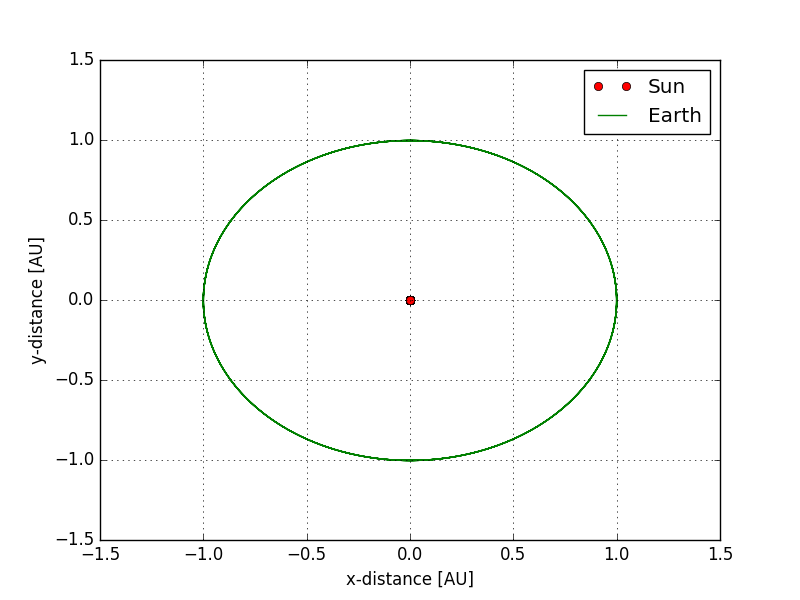
\includegraphics[width=\textwidth]{earth_sun_verlet_5years_dt0_001.png}
		\caption{Earth-Sun system over 5 years, calculated with velocity Verlet with $dt = 0.001$.}
		\label{fig:s_s_verlet_5yr_dt0_001}
	\end{subfigure}
	\caption{Forward Euler and velocity Verlet for 5 years at different timesteps.}
    \label{fig:euler_vs_verlet_5yr}
\end{figure}

\newpage

\begin{figure}
	\centering
	\begin{subfigure}[b]{0.4\textwidth}
		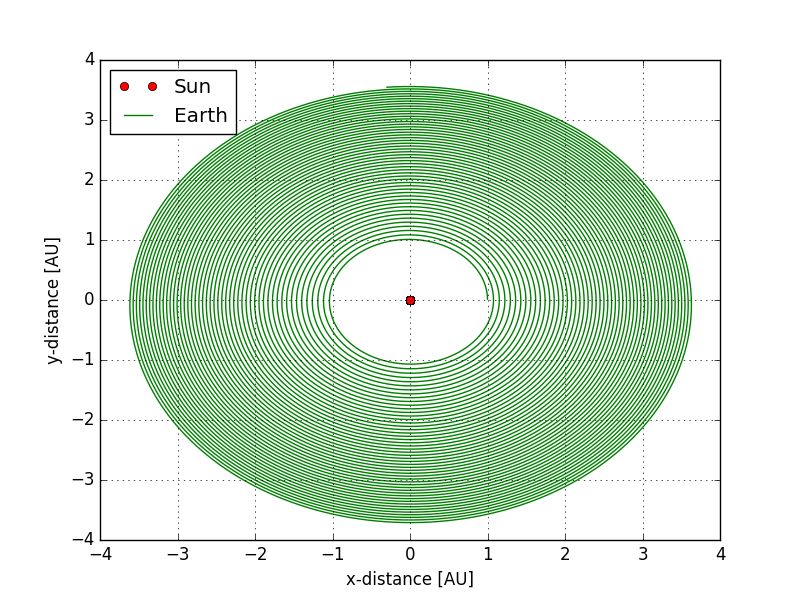
\includegraphics[width=\textwidth]{earth_sun_200yr_euler.png}
		\caption{Earth-Sun system over 200 years, calculated with forward Euler.}
		\label{fig:e_s_euler}
	\end{subfigure}
    \begin{subfigure}[b]{0.4\textwidth}
		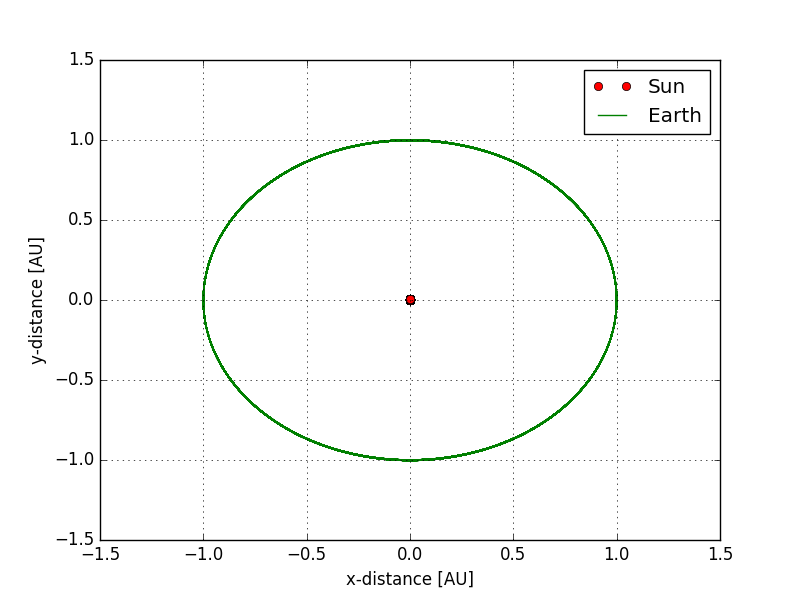
\includegraphics[width=\textwidth]{earth_sun_200yr_verlet.png}
		\caption{Earth-Sun system over 200 years, calculated with velocity Verlet.}
		\label{fig:e_s_verlet}
	\end{subfigure}
	\caption{Forward Euler and velocity Verlet over 200 years.}
    \label{fig:euler_vs_verlet}
\end{figure}

%
%\begin{figure}
%    \begin{subfigure}[b]{0.4\textwidth}
%		\includegraphics[width=\textwidth]%{solar_system_200yr_euler.png}
%		\caption{Solar system over 200 years, calculated with %forward Euler.}
%		\label{fig:s_s_euler}
%	\end{subfigure}
%	\begin{subfigure}[b]{0.4\textwidth}
%		\includegraphics[width=\textwidth]%{solar_system_200yr_verlet.png}
%		\caption{Solar system over 200 years, calculated with %velocity Verlet.}
%		\label{fig:s_s_verlet}
%	\end{subfigure}
    %\caption{All three methods for n = 10}
%\end{figure}


\begin{table}[h]
\centering
\caption{Energy and angular momentum conservation for the forward Euler and velocity Verlet methods for the Earth-Sun system. The energy is given in units [$\mathrm{M_\odot AU/yr^2}$], and the angular momentum in [$\mathrm{M_\odot AU^2/yr}$].}
\label{tab:euler_vs_verlet_earth_sun}
\begin{tabular}{l|l|l|l|l}
                       & FE, Earth-Sun     & VV, Earth-Sun\\  
\hline
E before    & $-5.92175\times 10^{-5}$            & $-5.92175\times10^{-5}$            \\
E after     & $-1.6245\times 10^{-5}$             & $-5.92175\times10^{-5}$             \\

\textbf{L} before & $1.88496\times 10^{-5}$\textbf{$e_z$} & $1.88496\times 10^{-5}$\textbf{$e_z$}\\
\textbf{L} after   & $3.59773\times 10^{-5}$\textbf{$e_z$}        & $1.88496\times 10^{-5}$\textbf{$e_z$}
\end{tabular}
\end{table}

\begin{comment}
\begin{table}[h]
\centering
\caption{Energy and angular momentum conservation for the forward Euler and velocity Verlet methods for the solar system.}
\label{tab:euler_vs_verlet_solar}
\begin{tabular}{l|l|l|l|l}
                       &  FE, Solar System        & VV, Solar System      \\
\hline
E before    & $-4.54826\times10^{-3}$            & $-4.54826\times10^{-3}$            \\
E after      & $-4.09022\times10^{-3}$            & $-4.54825\times10^{-3}$            \\

\textbf{L} before & $2.27612\times10^{-2}$\textbf{$e_z$} & $2.27612\times10^{-2}$\textbf{$e_z$} \\
\textbf{L} after   & $2.27612\times10^{-2}$\textbf{$e_z$} & $2.35448\times10^{-2}$\textbf{$e_z$}
\end{tabular}
\end{table}
\end{comment}


The forward Euler method and velocity Verlet method both use $5N + N^2$ FLOPS, where $N$ is the number of celestial objects we use.

When taking the time of both methods over 200 years with $dt = 0.00001$, the forward Euler method used $13.5061$ seconds to run, while the velocity Verlet method used $13.3799$ seconds.

\subsection{Escape Velocity}
\begin{figure}
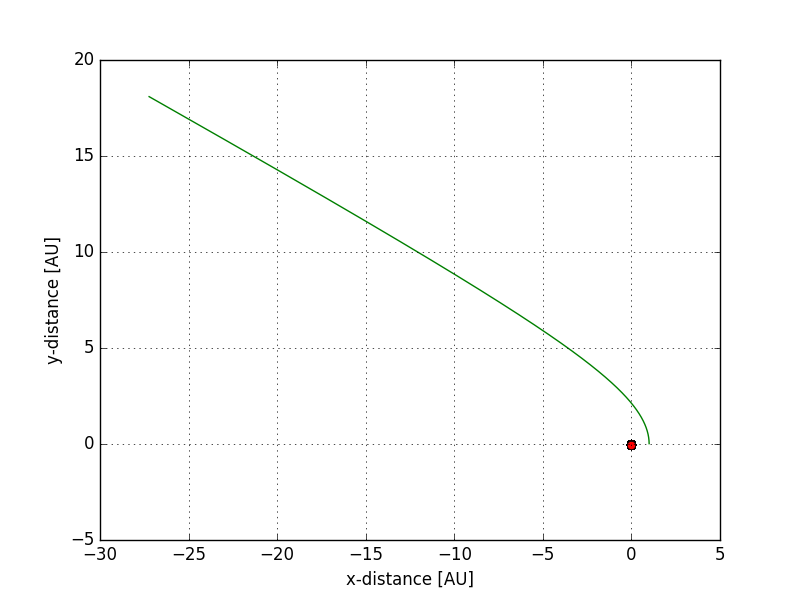
\includegraphics[width = \linewidth]{escape_velocity}
\caption{Earth escaping the magnetic pull of the Sun with an initial velocity of $2.9\pi$AU/yr in the direction of the Solar orbit. 10 year simulation.}
\label{fig:escape_velocity}
\end{figure}

The experimental results we got for the actual direction of the Earth velocity gave us an escape velocity of about $2.9\pi \mathrm{AU/yr}$. Compared to the analytical result we can see that we would need about 50\% more velocity to escape the pull of the Sun when moving perpendicular, rather than directly away from it. The plot we get when using this velocity can be seen in Figure \ref{fig:escape_velocity}.

\subsection{The Three-Body System}

\begin{figure}
	\centering
	\begin{subfigure}[b]{0.4\textwidth}
		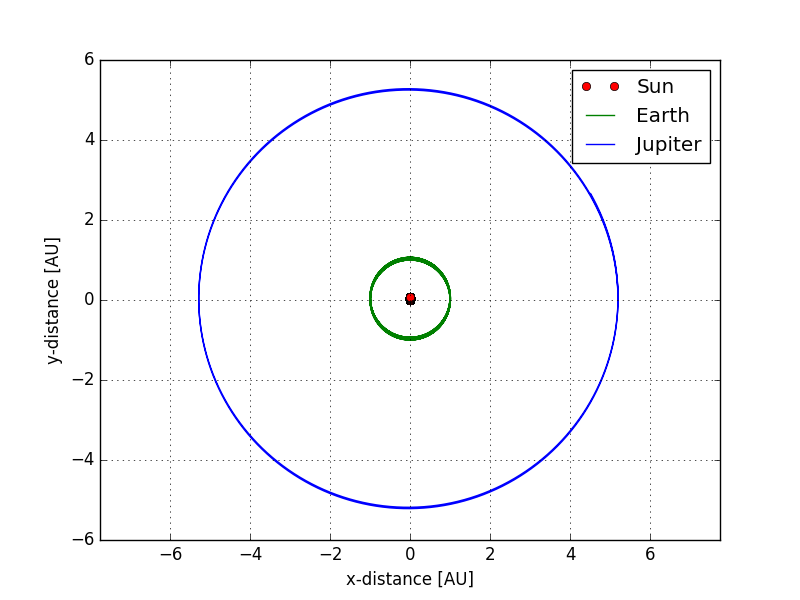
\includegraphics[width=\textwidth]{earth_sun_jupiter_verlet_25yr_dt0_00001_MJ1.png}
		\caption{All objects have their normal mass.}
		\label{fig:e_s_j_dt0_00001_m1}
	\end{subfigure}
	
	
    \begin{subfigure}[b]{0.4\textwidth}
		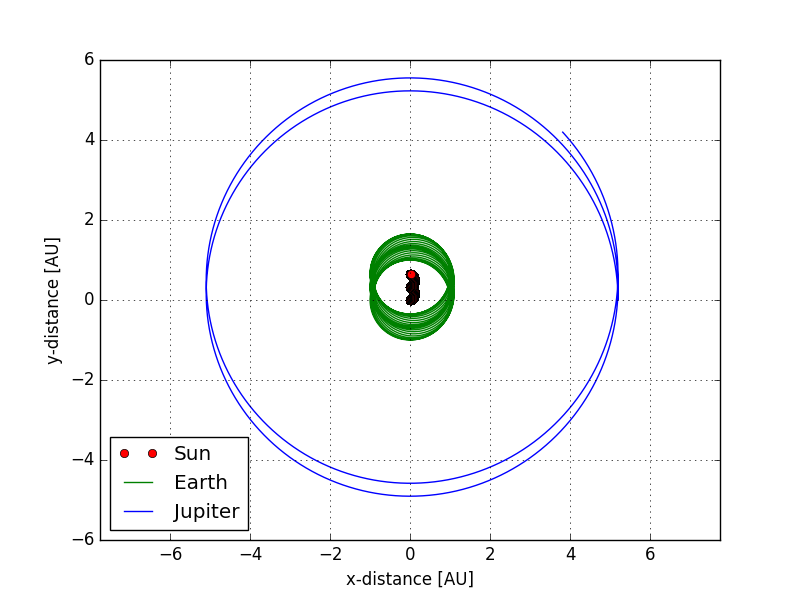
\includegraphics[width=\textwidth]{earth_sun_jupiter_verlet_25yr_dt0_00001_MJ10.png}
		\caption{Jupiter's mass multiplied by 10.}
		\label{fig:e_s_j_dt0_00001_m10}
	\end{subfigure}
	
	
    \begin{subfigure}[b]{0.4\textwidth}
		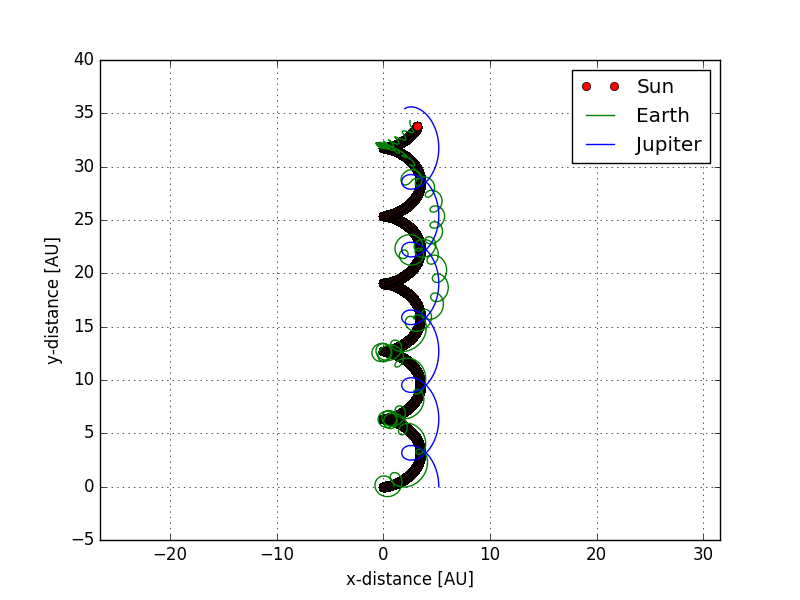
\includegraphics[width=\textwidth]{earth_sun_jupiter_verlet_25yr_dt0_00001_MJ1000.png}
		\caption{Jupiter's mass multiplied by 1000.}
		\label{fig:e_s_j_dt0_00001_m1000}
	\end{subfigure}
	\caption{Earth-Sun-Jupiter system over 25 years, calculated with velocity Verlet with a timestep $dt = 0.00001$.}
    \label{fig:e_s_j_25yr}
\end{figure}

Figure \ref{fig:e_s_j_25yr} shows the three-body system of the Earth, the Sun and Jupiter for various masses of Jupiter.


\begin{table}[]
\centering
\caption{Energy and angular momentum conservation for the Earth-Sun-Jupiter system for various masses of Jupiter over 25 years. The energy is given in units [$\mathrm{M_\odot AU/yr^2}$], and the angular momentum in [$\mathrm{M_\odot AU^2/yr}$].}
\label{tab:jupiter_mass_energies}
\begin{tabular}{l|l|l|l}
                                    & Real $M_J$      & 10 $M_J$  & 1000 $M_J$ \\
\hline
Total E before                 & $-3.818\times 10^{-3}$ & $-3.765\times 10^{-2}$ & $-3.75879$              \\
Total E after                  & $-3.818\times 10^{-3}$ & $-3.765\times 10^{-2}$ & $-3.7589$               \\
Total L before, $e_z$ & $1.442\times 10^{-2}$  & $1.44\times 10^{-1}$   & $14.398$                \\
Total L after, $e_z$   & $1.442\times 10^{-2}$  & $1.44\times 10^{-1}$   & $14.398$               
\end{tabular}
\end{table}

\subsection{Solar System}
\begin{figure}
	\centering
	\begin{subfigure}[b]{0.4\textwidth}
		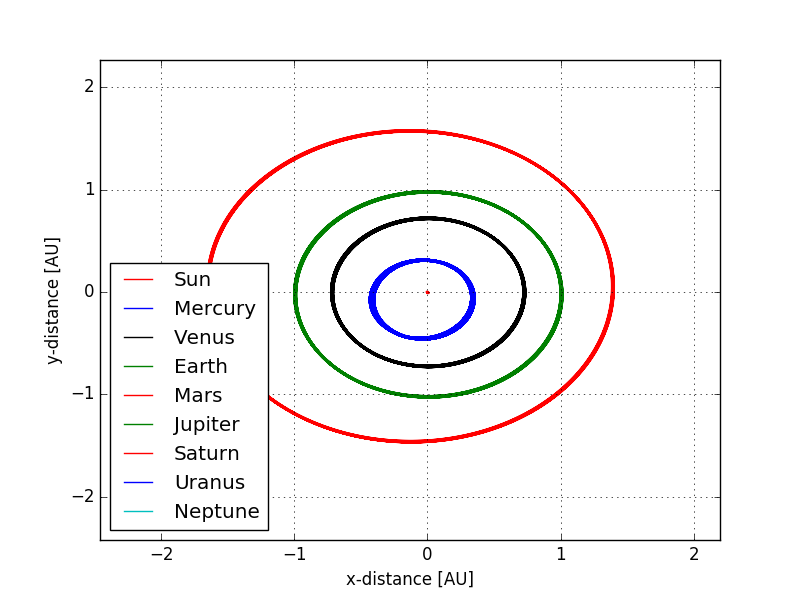
\includegraphics[width = \linewidth]{system_close}
		\caption{The inner solar system from Mars and inwards. Notice the thickness of the lines showing that the orbits are changing slightly over time.}
		\label{fig:system_all_a}
	\end{subfigure}
	
    \begin{subfigure}[b]{0.4\textwidth}
		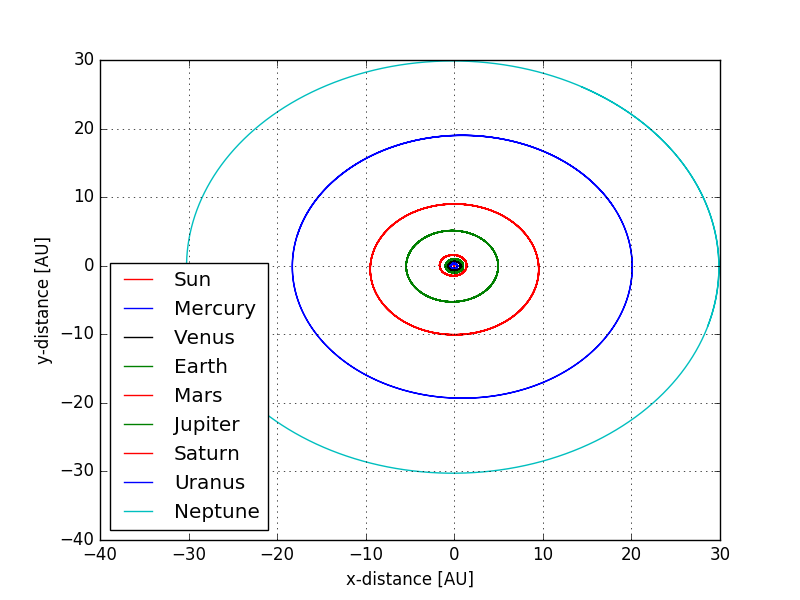
\includegraphics[width = \linewidth]{system_all}
		\caption{The inner green circle is Jupiter.}
		\label{fig:system_all_c}
	\end{subfigure}
	
	
    \begin{subfigure}[b]{0.4\textwidth}
		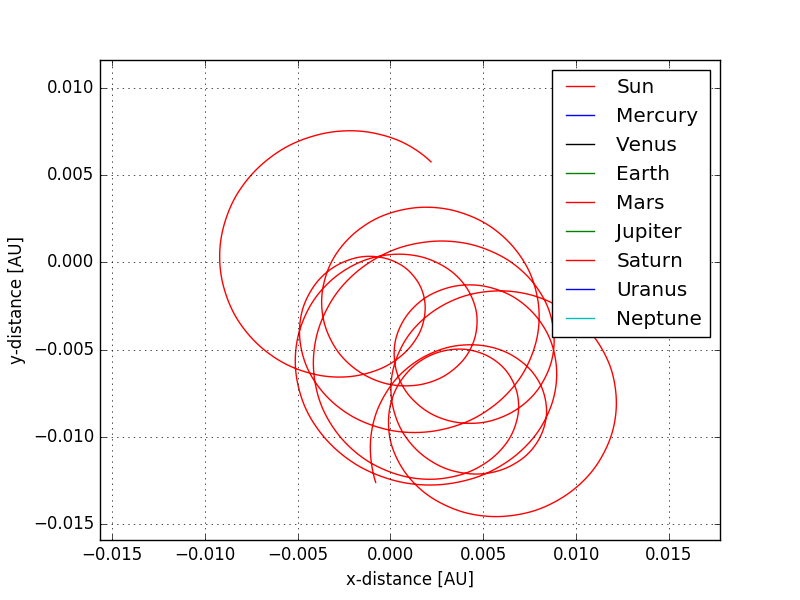
\includegraphics[width = \linewidth]{sun_complete}
		\caption{The motion of the sun zoomed in, using the model for the entire solar system.}
		\label{fig:system_all_b}
	\end{subfigure}
	
	\caption{The entire solar system moving for 200 years using the data aquired from the NASA website. Timestep $dt = 0.00001$.}
    \label{fig:system_all}
\end{figure}
We pulled the data of all the initial positions and velocities from the NASA website and used them to make a realistic model of a solar system containing only the sun and the 8 planets. This model can be seen in Figure \ref{fig:system_all}. 


\section{Conclusions and Discussion}

\subsection{Forward Euler and Velocity Verlet}

As seen in figure \ref{fig:euler_vs_verlet_5yr}, both the forward Euler and the velocity Verlet method works fine for this relatively small time period with a timestep of $dt = 0.00001$. However, in order to make the program run quicker, one would be inclined to increase the timestep. As we can see, for $dt = 0.001$, the velocity Verlet method stays the same, while the forward Euler becomes unstable, and the orbit increases. This can also be seen in figures \ref{fig:e_s_euler} and \ref{fig:e_s_verlet} - the velocity Verlet method stays stable.

If we look at table \ref{tab:euler_vs_verlet_earth_sun}, we can see that the forward Euler method does not properly conserve energy and angular momentum. We decided to look for conservation of total momentum, instead of the individual kinetic and potential. The reason is that if the total energy is conserved, we know that the method is stable.

We also calculate the angular momentum. Table \ref{tab:euler_vs_verlet_earth_sun} shows clearly that after 200 years, the velocity Verlet method completely conserves angular momentum in z-direction (which all our angular momentum will be in, since we approximate the momevent to be in the xy-plane) - at least down to the 5th decimal. The forward Euler method, however, has almost doubled the angular momentum over the 200 years.

As long as the planet is in a stable circular orbit, these quantities should stay the same. A change of energy or angular momentum would mean a change in velocity, which would mean a change in radius. In other words, if energy and angular momentum is not conserved, the planets would either spiral into the Sun or off into the void. We know that in our solar system this is not the case, so we must make sure our program conserves these quantities.

By comparing the two methods, velocity Verlet seems to be strictly superior. It uses the same ammounts of FLOPS as forward Euler, runs a little bit faster, and is much more precise. According to our results there is no redeeming qualities to forward Euler at all compared to velocity Verlet, at least for this kind of system.

As seen in figures \ref{fig:euler_vs_verlet_5yr} and \ref{fig:euler_vs_verlet}, the Verlet method is idiotically stable compared to the forward Euler. Especially \ref{fig:euler_vs_verlet} shows that after 200 years, the same computations that are completely stable with velocity Verlet has given the earth an orbit that is almost four times greater with the forward Euler method.

\subsection{The Earth-Sun System}

As we can see in figures \ref{fig:euler_vs_verlet_5yr} and \ref{fig:euler_vs_verlet}, the two-body system seems very stable for the velocity Verlet method, and less so for the forward Euler method when the timestep is not small enough.

The object-oriented code seems to work as intended. It runs fairly fast, and it is simple to add more objects. It should be no trouble adding even more celestial objects if desired, such as Pluto and the moons of the planets.

\subsection{The Three-Body System}

Figure \ref{fig:e_s_j_25yr} shows the three-body system of the Earth, the Sun and Jupiter for various masses of Jupiter.

In figure \ref{fig:e_s_j_dt0_00001_m1}, with the normal Jupiter mass, the result is pretty much as expected. The orbits go as usual.

When we multiply the mass of Jupiter by 10, things get more interesting, as seen in figure \ref{fig:e_s_j_dt0_00001_m10}. Jupiter now has a clearly visisble attraction on the orbits of the Earth and the Sun. This also seems to destabilize the orbits of all objects. They do appear to still be somewhat circular in shape, but the circles seem to "move".

Figure \ref{fig:e_s_j_dt0_00001_m1000} shows what happens when Jupiter has its mass multiplied by 1000, that is, when it's in the same order of maginude as the Sun. Now we basically have a double-star system, with a single planet orbiting both.

As we can see in table \ref{tab:jupiter_mass_energies} the energies and angular momentums are still very well conserved. As we can see, the only loss of precision is in the fourth decimal of the energy when the mass is 1000 times normal. To see if this error evolved further, we ran the program for 250 and 2500 years. For 250 years we got $E = -3.65732 \mathrm{M_\odot AU/yr^2}$. As we can see, the error has now evolved up to the first decimal. However, when running for 2500 years, the energy is $E = -3.65752 \mathrm{M_\odot AU/yr^2}$. The error is still in the first decimal, but if we look at the third decimal, the error has gotten smaller again. This indicates that while the Verlet method may give us a small error during extreme conditions, it will stabilize itself again.

All in all this shows that we can be really confident about the stability of the velocity Verlet method.

However, because we use the sun as the centre of mass, and Jupiter will have a pull on the sun, the whole system will be pulled in the direction of Jupiter's initial velocity.

\subsection{Solar System}

As you can see in Figure \ref{fig:system_all}, the lines in the inner solar system are thicker than the lines in the outer solar system. This is because the orbit of the planets change slightly over time, and the inner planets have have shorter orbital periods around the Sun than the outer planets, broadening the lines as the orbits change. In time, this will also be visible for the outer planets. 



\section{Extra Material}
You can find the code we used to calculate these results at: 

\begin{thebibliography}{99}
%\bibitem{taut}\href{http://prola.aps.org/abstract/PRA/v48/i5/p3561_1}{M. Taut, Phys. Rev. A 48, 3561 (1993)}
%\bibitem{jensen} M.~H.̃~Jensen, Computational~Physics(11.09.2017) \url{github.com/CompPhysics/ComputationalPhysics/blob/master/doc/Projects/2017/ReportExamplesLatexstyle/reportexample.tex}
\end{thebibliography}

\end{document}